\subsection*{Teil B: Körper und ihre Eigenschaften (25 Minuten)}

\begin{enumerate}[label=\arabic*.,resume]

    \item \textbf{Symmetrien identifizieren:}

    Welche Symmetrien haben die folgenden Körper? Kreuze an!

    \begin{center}
        \begin{tabular}{|l|c|c|c|}
            \hline
            \textbf{Körper} & \textbf{Symmetrieachse} & \textbf{Symmetrieebene} & \textbf{Symmetriezentrum} \\
            \hline
            Würfel & $\square$ & $\square$ & $\square$ \\
            \hline
            Kugel & $\square$ & $\square$ & $\square$ \\
            \hline
            Zylinder & $\square$ & $\square$ & $\square$ \\
            \hline
            Kegel & $\square$ & $\square$ & $\square$ \\
            \hline
        \end{tabular}
    \end{center}

    \vspace{1cm}

    \item \textbf{Rotationskörper erkennen:}

    Welcher Körper entsteht, wenn die Figur um die eingezeichnete Achse rotiert?

    \begin{center}
        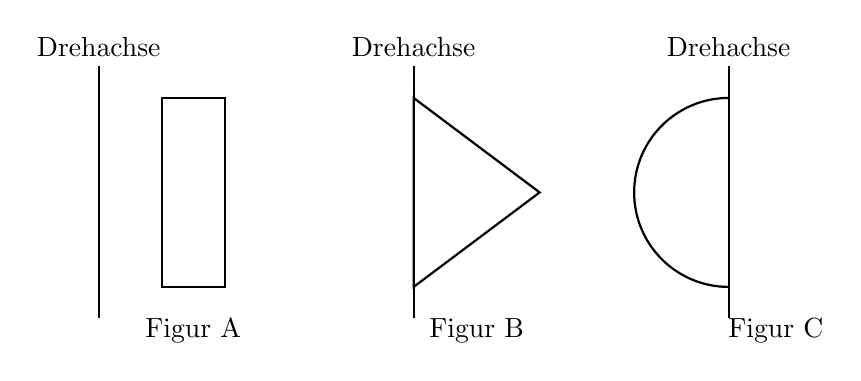
\begin{tikzpicture}[scale=0.8]
        % Rechteck um y-Achse
        \draw[thick] (0,-2) -- (0,2) node[above]{Drehachse};
        \draw[thick] (1,-1.5) rectangle (2,1.5);
        \node at (1.5,-2.2) {Figur A};

        % Dreieck um Seite
        \begin{scope}[xshift=5cm]
            \draw[thick] (0,-2) -- (0,2) node[above]{Drehachse};
            \draw[thick] (0,-1.5) -- (2,0) -- (0,1.5) -- cycle;
            \node at (1,-2.2) {Figur B};
        \end{scope}

        % Halbkreis um Durchmesser
        \begin{scope}[xshift=10cm]
            \draw[thick] (0,-2) -- (0,2) node[above]{Drehachse};
            \draw[thick] (0,-1.5) arc (270:90:1.5);
            \node at (0.75,-2.2) {Figur C};
            \end{scope}
        \end{tikzpicture}
    \end{center}

    Figur A ergibt: \underline{\hspace{4cm}} \hspace{1cm}
    Figur B ergibt: \underline{\hspace{4cm}} \hspace{1cm}
    Figur C ergibt: \underline{\hspace{4cm}}

    \vspace{1cm}

    \item \textbf{Axialschnitte zeichnen:}

    Zeichne den Axialschnitt der folgenden Rotationskörper:

    \begin{center}
        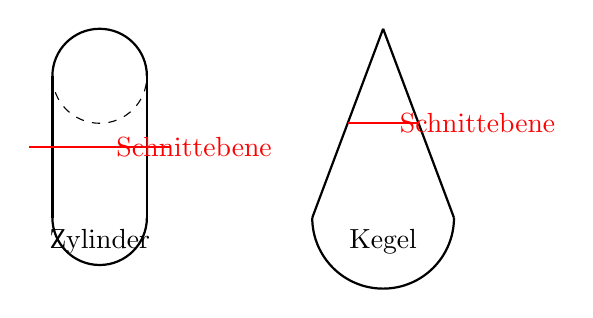
\begin{tikzpicture}[scale=0.6]
            % Zylinder
            \begin{scope}
                \draw[thick] (-1,0) arc (180:360:1);
                \draw[thick] (-1,0) -- (-1,3);
                \draw[thick] (1,0) -- (1,3);
                \draw[thick] (-1,3) arc (180:0:1);
                \draw[dashed] (-1,3) arc (180:360:1);
                \node at (0,-0.5) {Zylinder};
                \draw[red, thick] (-1.5,1.5) -- (1.5,1.5);
                \node[red] at (2,1.5) {Schnittebene};
            \end{scope}

            % Kegel
            \begin{scope}[xshift=6cm]
                \draw[thick] (-1.5,0) arc (180:360:1.5);
                \draw[thick] (-1.5,0) -- (0,4);
                \draw[thick] (1.5,0) -- (0,4);
                \node at (0,-0.5) {Kegel};
                \draw[red, thick] (-0.75,2) -- (0.75,2);
                \node[red] at (2,2) {Schnittebene};
            \end{scope}
        \end{tikzpicture}
    \end{center}

    Zeichne hier die Axialschnitte:

    \vspace{4cm}

\end{enumerate}
